\chapter{Implementação da Solução}
\label{sec:4-Implementacao}

Este capítulo aprofunda o processo de desenvolvimento da solução para o problema do projeto em 
análise de acordo com a análise e os princípios de \textit{design} discutidos no capítulo anterior. 
Além disso, é efetuada uma análise cuidada dos resultados obtidos através das decisões anteriores, 
revelando os resultados consequentes e a sua concordância com os objetivos discutidos anteriormente.

\section{Tecnologias Utilizadas}

Durante o desenvolvimento do projeto, foram utilizadas várias tecnologias e ferramentas para a 
implementação da solução. Entre as mais relevantes, destacam-se:

\begin{itemize}
  \item \textbf{Apache Storm \cite{storm}:} \textit{Framework} de processamento de 
    \textit{streaming} em tempo real;
  \item \textbf{Apache Kafka \cite{kafka}:} Plataforma de mensagens distribuída;
  \item \textbf{Apache Zookeeper \cite{zookeeper}:} Serviço de coordenação distribuída;
  \item \textbf{Grafana \cite{grafana}:} Plataforma de análise e visualização de dados;
  \item \textbf{Jenkins \cite{jenkins}:} Servidor de automação de \textit{builds}; 
  \item \textbf{Nimbus \cite{nimbus}:} Servidor centralizado que coordena e distribui as topologias 
    do \textit{Apache Storm};
  \item \textbf{Splunk \cite{splunk}:} Plataforma de análise de eventos e dados;
\end{itemize}

\section{Descrição da implementação}

De forma a conseguir atingir os objetivos pretendidos, analisados no capítulo anterior, é
necessário ter em conta vários processos que fazem parte da implementação da solução. Para 
facilitar a compressão e análise dos mesmos vão ser apresentados os vários passos e algum 
suporte, como diagramas, que ajudam a ter uma melhor compreensão de todo o processo necessário
para atingir estes objetivos.

\subsection{Processo de \ac{CI} de um serviço}

Cada serviço é composto, normalmente, por três componentes principais, como ilustrado na Figura
\ref{package}, separados em diferentes repositórios. Os três componentes habituais de um novo 
serviço são: o código do serviço - o código com toda a lógica de programação que compõe o serviço, 
configurações do pacote - repositório com as configurações do serviço, como versões de serviços 
externos necessários nas \acp{VM} que são necessárias para o serviço, esta componente usa 
ferramentas de configuração como Chef \cite{chef} ou Ansible \cite{ansible} e, por fim, um 
repositório com configurações relativamente à infraestrutura - repositório com as configurações de 
infraestrutura necessárias para o serviço, como especificações dos \glspl{flavour} e das 
\textit{subnets} necessárias.

\begin{figure}[H]
  \centerline{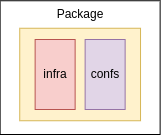
\includegraphics[scale=1.2]{media/content/impl/package.png}}
  \caption{Composição típica do pacote de um serviço}
  \label{package}
\end{figure}

Todo o processo de \ac{CI} é gerido pelo Jenkins, que é responsável por criar os artefactos
necessários para a execução do serviço nos ambientes que estão ativos. A Figura \ref{ci-process} 
ilustra, de uma forma simplificada, o processo de \ac{CI} de um serviço.

\todo[inline]{TODO: Falar sobre packages jenkins e i2 e a integração com jobs e pipelines}
 
% \begin{figure}[H]
%   \centerline{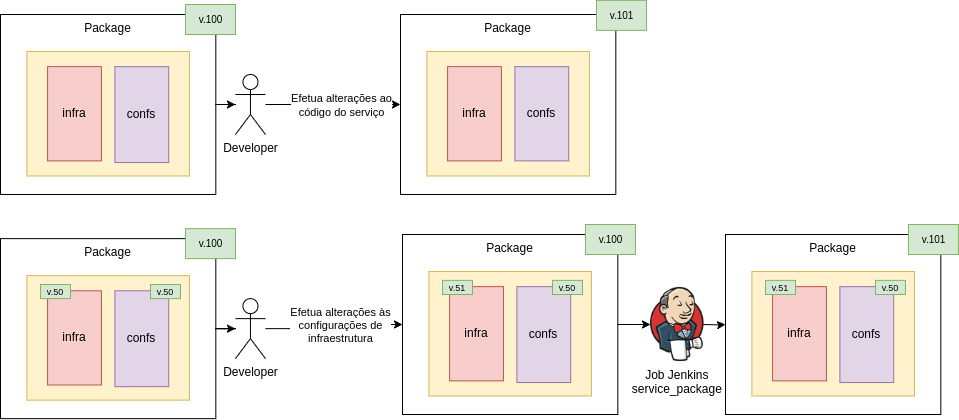
\includegraphics[scale=0.12]{media/content/impl/ci-process.png}}
%   \caption{Processo de \ac{CI} de um serviço}
%   \label{ci-process}
% \end{figure}

\subsection{\textit{Scaledown} do Cluster}

Um dos processos necessários para conseguir atingir a solução pretendida é efetuar a alteração
de configurações do uso de recursos (\gls{flavour}) dos \glspl{cluster} existentes. Como
referido anteriormente todos os processos de infraestrutura são geridos internamente pela Blip e,
desta forma, têm os seus processos próprios para este tipo de operações.

Neste caso, as configurações dos recursos dos serviços é efetuado a partir de um repositório 
de configurações específicas de infraestrutura para cada um dos serviços. Ao efetuar uma alteração
neste repositório é automaticamente despoletado um Job Jenkins que trata da criação do artefacto
da nova versão e executa a \textit{pipeline} correspondente no ambiente de \ac{QA}.

Todo este processo é automatizado e, por isso, é necessário compreender quais são os mecanismos
existentes de forma a trabalhar de forma eficiente com os mesmos. A Figura \ref{scaledown-nxt} 
ilustra o processo de \textit{scaledown} de um \textit{cluster} no ambiente de NXT e qual o 
procedimento adicional em caso de necessidade de reversão da operação.

\begin{figure}[H]
  \centerline{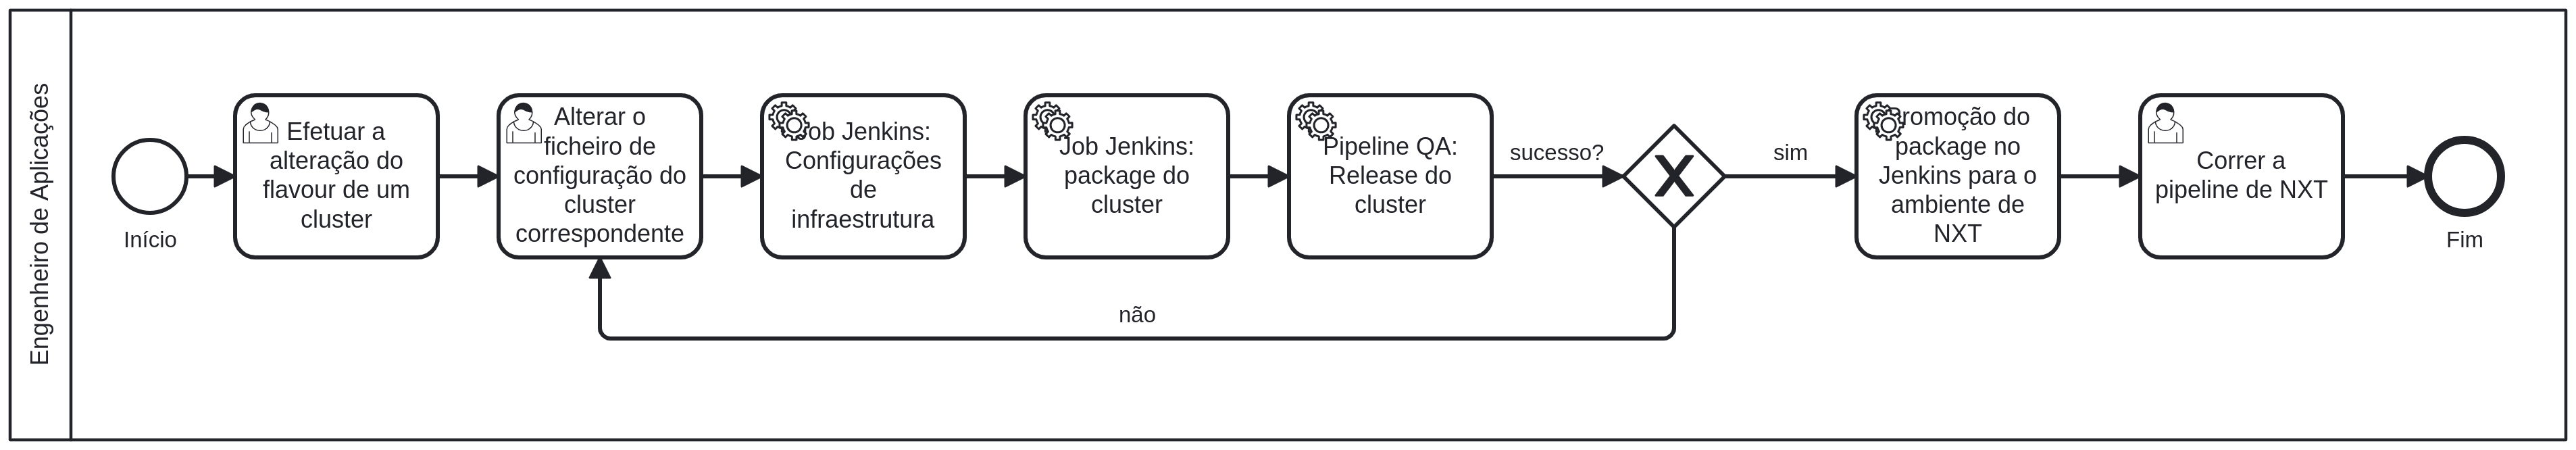
\includegraphics[scale=0.12]{media/content/impl/scaledown_nxt.png}}
  \caption{Processo de \textit{scaledown} de um \textit{cluster} no ambiente de NXT}
  \label{scaledown-nxt}
\end{figure}

\subsection{Criação de um Cluster}

\todo[inline]{Incluir BPMNs do processo de criação de novos clusters (simplificado}

\section{Testes}

De forma a testar a solução desenvolvida, foram efetuados vários testes, tanto por parte das
equipas de desenvolvimento, responsáveis por cada um dos serviços presentes no \gls{cluster},
como por parte da nossa equipa de operações. 

De um ponto de vista operacional, os testes efetuados foram focados na utilização geral de
recursos do \gls{cluster}. Para isso, foram efetuadas comparações entre os recursos utilizados
antes e depois da implementação da solução, utilizando testes de carga para simular situações
de utilização de recursos exigentes.

Como a redução inicial teve por base apenas a redução do \gls{flavour} do \ac{CPU}, vamos ter em conta
apenas essa métrica. Como é possível observar na Figura \ref{usage-before}, a utilização de \ac{CPU}
do \gls{cluster} antes da implementação ronda os 20\% de uso total.

\begin{figure}[H]
  \centerline{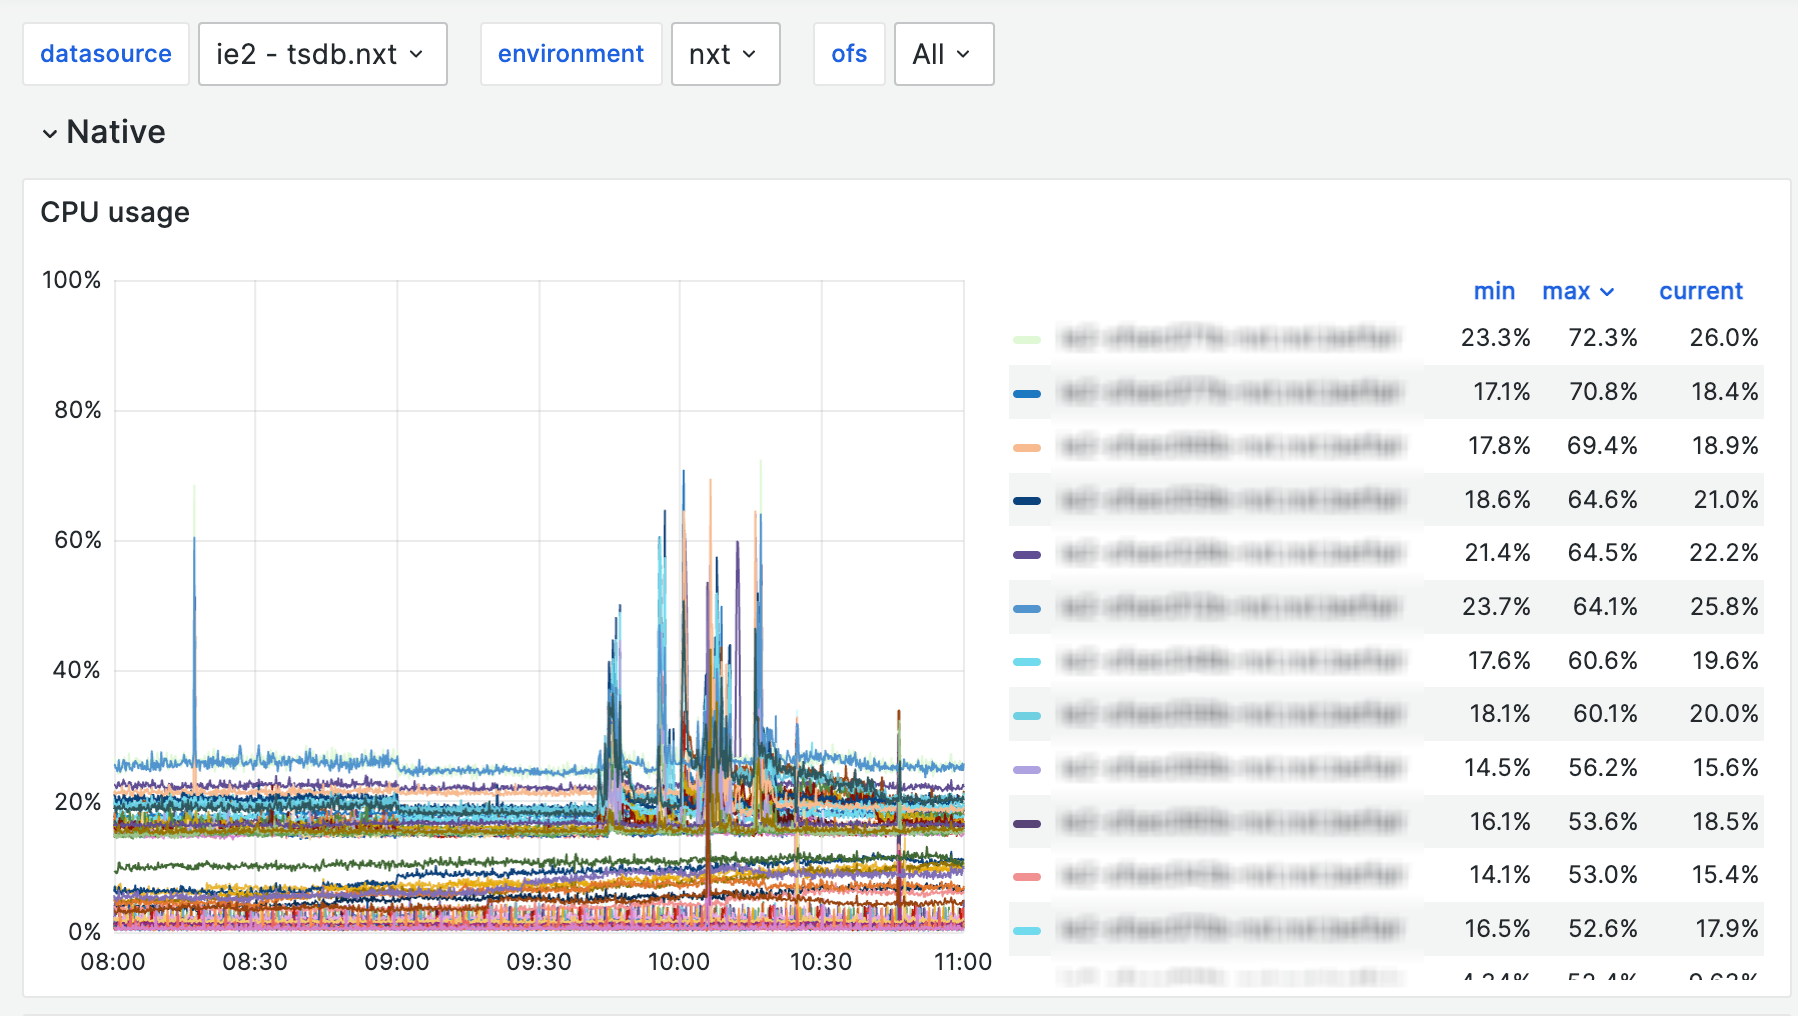
\includegraphics[scale=0.25]{media/content/impl/grafana-before-1.png}}
  \caption{Utilização de recursos do \textit{cluster} antes da implementação da solução}
  \label{usage-before}
\end{figure}

Após a redução de recursos inicial é possível verificar que o uso aumentou para os 40\%, um aumento
no nível esperado dada a alteração que foi efetuada. É importante, perceber que o \gls{cluster}
mantém a sua capacidade de processar dados em momentos de carga elevada de forma a poder concluir
que esta alteração não vai impactar negativamente o desempenho percetível do sistema. 

\begin{figure}[H]
  \centerline{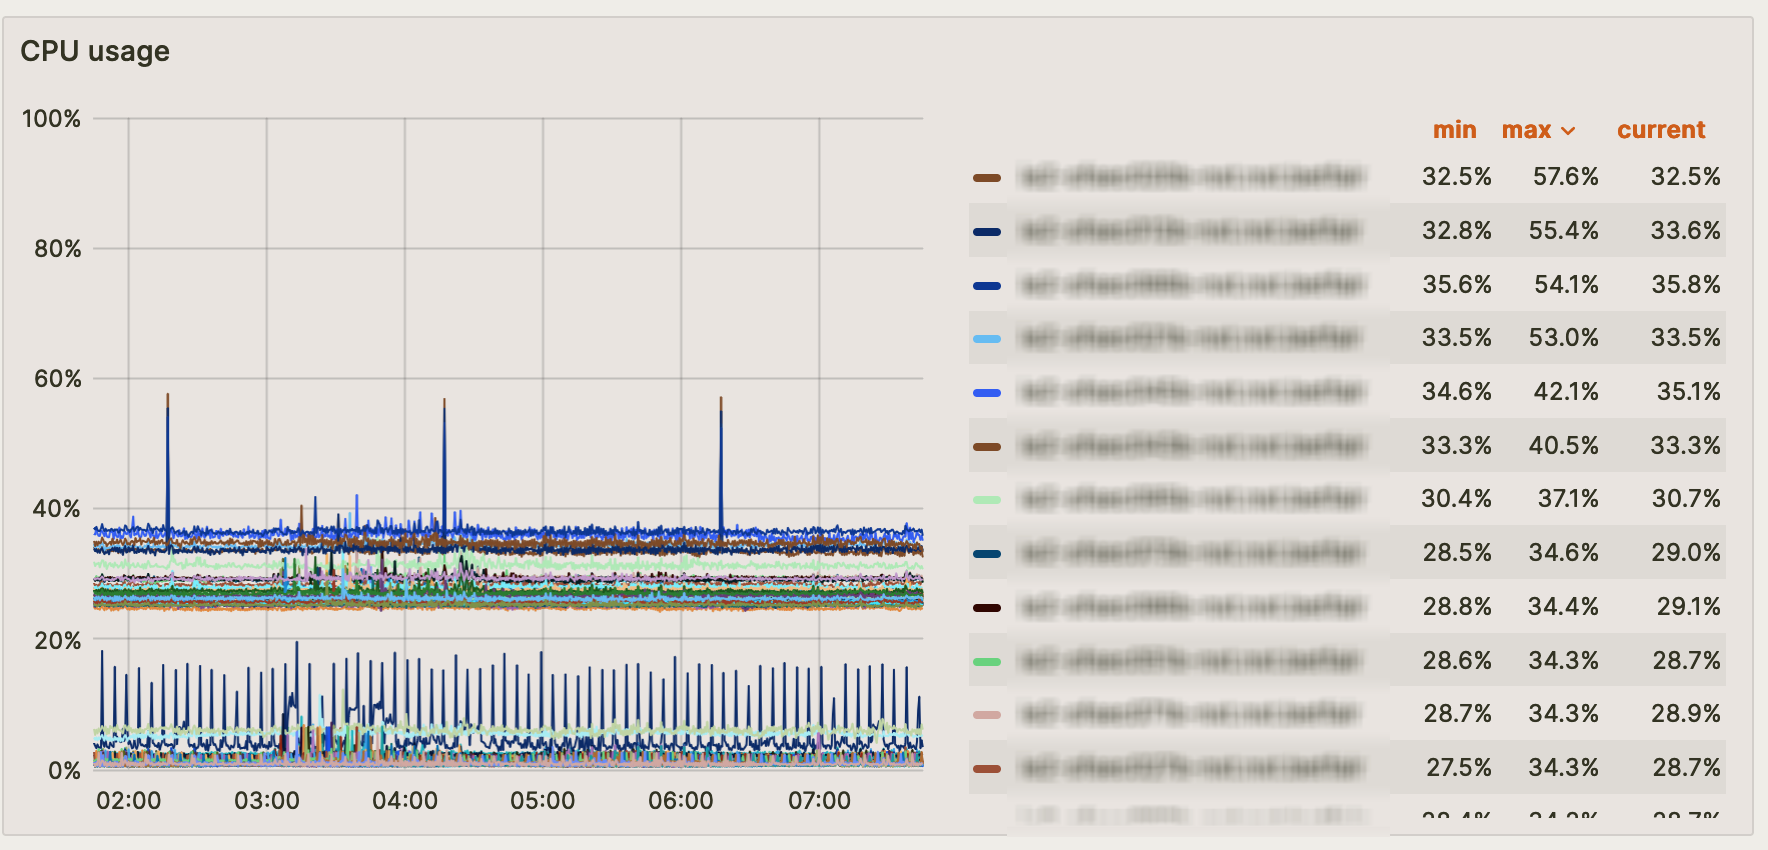
\includegraphics[scale=0.5]{media/content/impl/grafana-after.png}}
  \caption{Utilização de recursos do \textit{cluster} após a implementação da solução}
  \label{usage-after}
\end{figure}

\section{Avaliação da Solução}

\todo[inline]{TODO}

